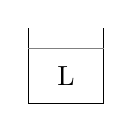
\begin{tikzpicture}[scale = 0.8]
  %%%%%%%%%%%%%The first bin%%%%%%%%%%%%%%%%%%%%%%
  \draw (0,1.2) -- (0,0) -- (1.2,0)--(1.2,1.2);
  \draw[gray] (0,0.88) -- (1.2,0.88);
  \draw (0.6,0.44) node {L};
\end{tikzpicture}
\quad
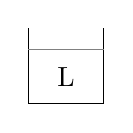
\begin{tikzpicture}[scale = 0.8]
  %%%%%%%%%%%%%The second bin%%%%%%%%%%%%%%%%%%%%%%
  \draw (0,1.2) -- (0,0) -- (1.2,0)--(1.2,1.2);
  \draw[gray] (0,0.86) -- (1.2,0.86);
  \draw (0.6,0.43) node {L};
\end{tikzpicture}
\quad
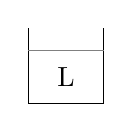
\begin{tikzpicture}[scale = 0.8]
  %%%%%%%%%%%%%The third bin%%%%%%%%%%%%%%%%%%%%%%
  \draw (0,1.2) -- (0,0) -- (1.2,0)--(1.2,1.2);
  \draw[gray] (0,0.84) -- (1.2,0.84);
  
  \draw (0.6,0.42) node {L};
\end{tikzpicture}
\hspace*{0.66em}\raisebox{-0.2em}{
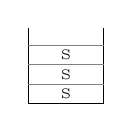
\begin{tikzpicture}[scale = 0.8]
  %%%%%%%%%%%%%The forth bin%%%%%%%%%%%%%%%%%%%%%%
  \draw (0,1.2) -- (0,0) -- (1.2,0)--(1.2,1.2);
  \draw[gray] (0,0.31) -- (1.2,0.31);
  \draw[gray] (0,0.62) -- (1.2,0.62);
  \draw[gray] (0,0.93) -- (1.2,0.93);
  
  \draw (0.6,0.155) node {\tiny{S}};
  \draw (0.6,0.465) node {\tiny{S}};
  \draw (0.6,0.775) node {\tiny{S}};
\end{tikzpicture}}